\chapter{The \texttt{BareBones.ino} Sketch}

I shall now present you with a small sketch which talks directly with \twi{} to setup, configure and read data from an LM75 sensor. The sketch doesn't make use of many of the features of the sensor, merely these two:

\begin{itemize}
    \item Reading the product id from the LM75. Some LM75s do not have the product id present. I believe only Texas Instruments' devices have it. Mine are NXP Semiconductor.
    \item Reading the current temperature.
\end{itemize}

\section{The Breadboard Layout}

Figure \ref{fig: BareBones.ino - Breadboard layout} (see Page \pageref{fig: BareBones.ino - Breadboard layout}) shows the circuit layout for the \path{BareBones.ino} sketch\footnote{And also, for the \path{WithLibrary.ino} sketch coming later!}.

\begin{figure}[!h]
\begin{centering}
    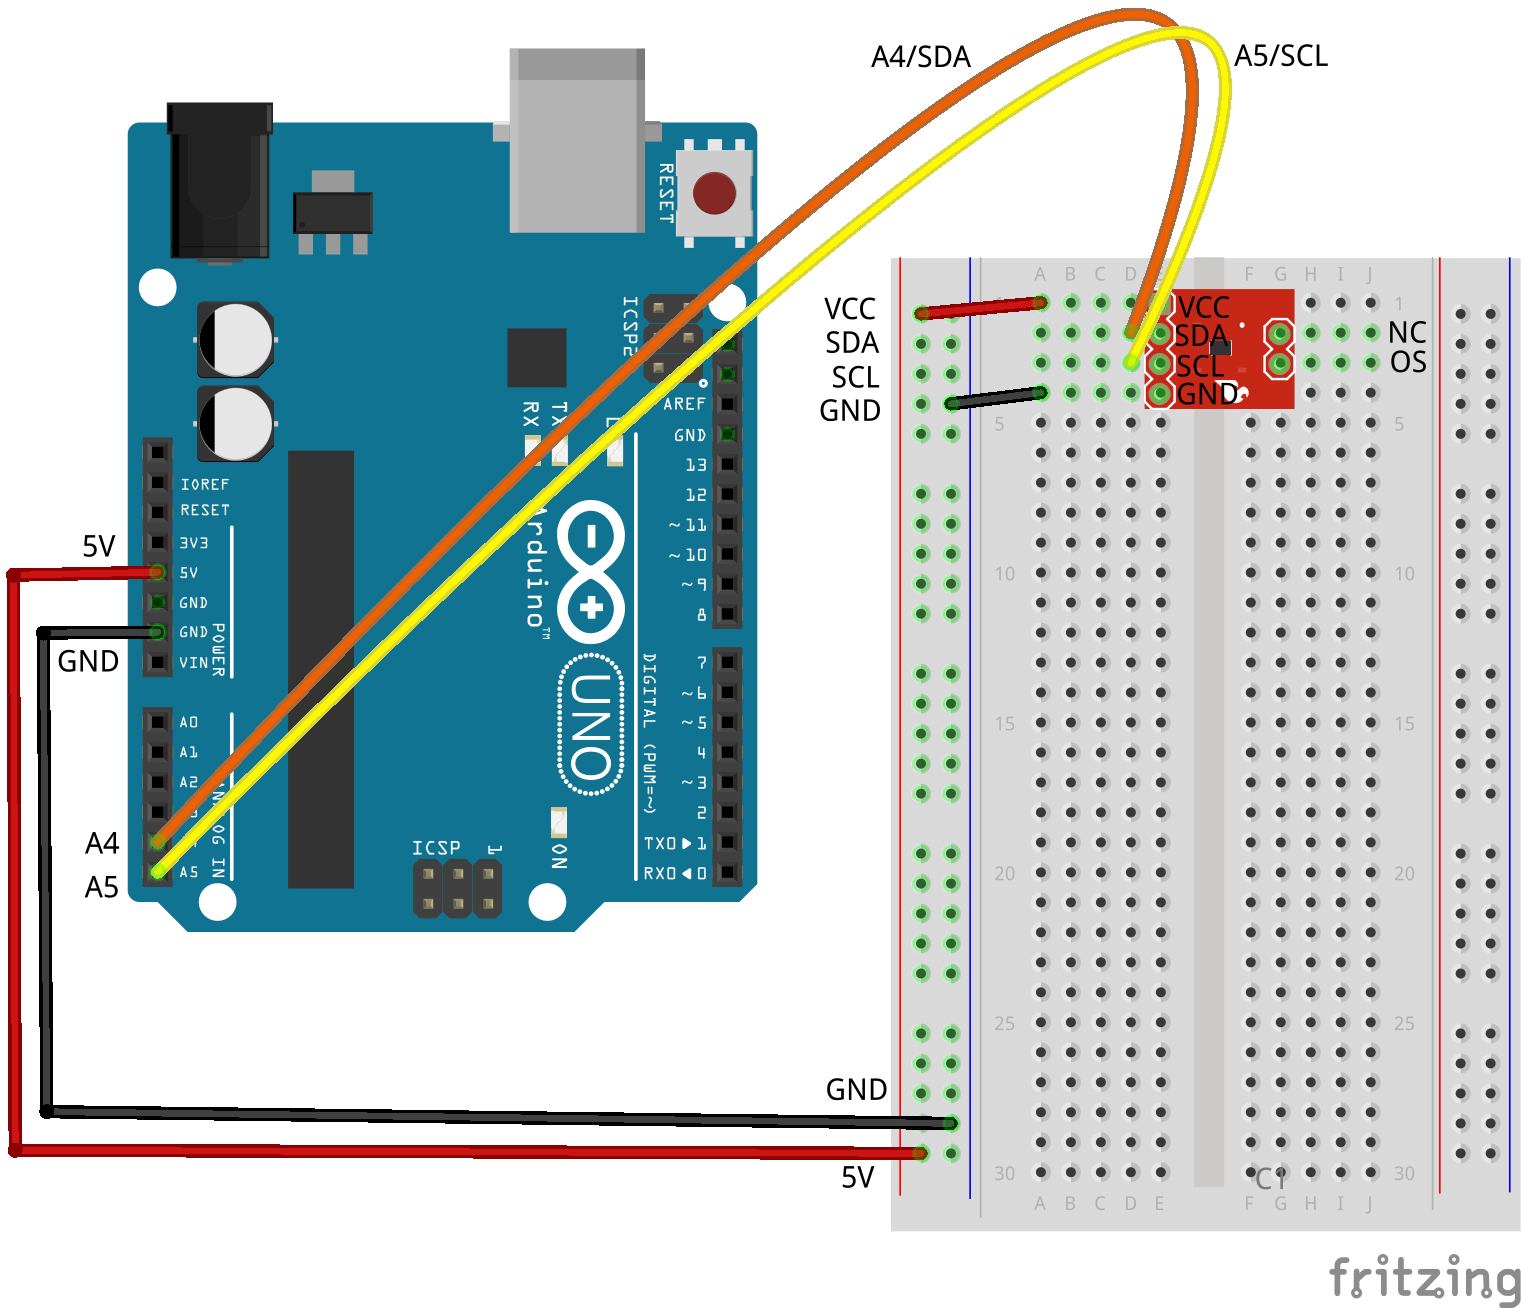
\includegraphics[width=11cm]{Fritzing/BareBones}
    \caption{BareBones.ino - Breadboard layout.}
    \label{fig: BareBones.ino - Breadboard layout}
    \par\end{centering}
\end{figure}

Power and ground connections go directly from the Arduino's power and ground pins, to the supply rails on the breadboard. The sensor's own \pin{VCC} and \pin{GND} pins take their power from the breadboard.

As we are using \twi{}, we have no choice in this matter as it's all the LM75 understands, we need two additional wires---one for the \twi{} bus clock and one for the \twi{} bus data.

On Figure \ref{fig: BareBones.ino - Breadboard layout} you will see the yellow and orange wires are connected to the Arduino's \pin{A5} and \pin{A4} pins respectively.

Other clones of the Arduino Uno, like mine, have two separate pins---\pin{SCL} and \pin{SDA}--- for the \twi{} bus clock and data pins. To avoid confusion, I'm using the same physical layout as shown in Figure \ref{fig: BareBones.ino - Breadboard layout}.

Unfortunately the Fritzing component image is slightly different to my own physical one, but the pins are the same names at least! (\pin{NC} is ``not connected''.)

Right, on with the code.

\section{Sketch Header}

It's always nice to start with a header giving details of what the sketch is doing and when you wrote it. You'd be surprised how often it helps! Here's mine, intentionally kept brief, having said that!

\begin{lstlisting}[caption={BareBones.ino - Header.},label={lst: BareBones.ino - Header}, style=myArduino, firstnumber=1]
//===============================================================
// LM75 Temperature sensor demo for MakerSpace presentation.
//
// Shows how much messing about with I2C/TWI there is in order
// to read the temperature and product id from an LM75A/B sensor.
//
// The LM75A/B can do a lot more than shown here, for the sake of
// brevity, I'm not getting in too deep!
//
//
// Norman Dunbar.
// 16 June 2026.
//===============================================================
\end{lstlisting}

\section{Sketch Prologue}

In the prologue for the sketch, I have included the \path{Wire.h} header file. This is required as I need to access the \twi{} bus.

Following on from that, I have declared the various LM75 accessing functions that will be used in the code. I do it this way as \func{setup()} and \func{loop()} will appear near the top of the listing and should be easier to find when making changes.

The functions declared will be at the bottom of the sketch and as such, the compiler needs to know about them so that when it finds calls to them, it knows how to handle things like parameters and return values.


\begin{lstlisting}[caption={BareBones.ino - Prologue.},label={lst: BareBones.ino - Prologue}, style=myArduino, firstnumber=15]
#include <Wire.h>


// Function prototypes.
void LM75_begin(const int address, uint32_t clockHZ);
void LM75_end();
void LM75_setRegister(const int address, const int reg);
uint8_t LM75_getProductId(const int address);
float LM75_getCurrentTemperature(const int address);


// Where is my sensor?
const int LM75_ADDRESS = 0x4F;

// Bus speed in Hz.
const uint32_t LM75_CLOCK_HZ = 100000;    // 100 KHz.

// LM75 registers.
const int LM75_TEMPERATURE_REG = 0;
const int LM75_PRODUCT_ID_REG = 7;

// Product id is unknown.
const uint8_t LM75_UNKNOWN_ID = 255;
\end{lstlisting}

Following on from the function prototypes, I have made life easy for myself by declaring constants for all the ``magic'' numbers that will appear in the code. If I ever have to make changes, I only need to find and change one value!



\section{Setup}

The Arduino standard \func{setup()} function is next. Not much happens here other than starting the \twi{} bus with a clock speed of 100~KHz and initialising the LM75 sensor attached to address \hexa{4F}---note that this is a seven bit address, not eight!

\eject\begin{tips}{Note}
    Internally, \twi{} uses an eight bit address which is determined by the device's seven bit address shifted left by one bit and a 0 (write) or a 1 (read) tagged onto the lowest bit.

    This gives my particular LM75 sensor a read address of \hexa{4F} \shl{1}|1 which is \hexa{9F}; and a write address of \hexa{4F} \shl{1}|1 which is \hexa{9E}. However, I only have to remember the seven bit address \hexa{4F}.
\end{tips}


\begin{lstlisting}[caption={BareBones.ino - Setup.},label={lst: BareBones.ino - Setup}, style=myArduino, firstnumber=43]
void setup() {
    uint8_t productID;

    // Start up I2C as a controller. Talking to the sensor
    // at 100 KHz.
    LM75_begin(LM75_ADDRESS, LM75_CLOCK_HZ);

    // Need the Serial Monitor for output.
    Serial.begin(9600);
    Serial.println("LM75 Temperature Sensor");
    Serial.print("LM75 Product id: ");

    productID = LM75_getProductId(LM75_ADDRESS);
    if (productID == LM75_UNKNOWN_ID)
    Serial.println("Unknown");
    else
    Serial.println(productID);
}
\end{lstlisting}

After initialising the LM75, Serial is initialised to 9600 baud and a message printed to show that we are starting up. The LM75's product id is fetched from the device and printed---if one is present. See Listing \ref{lst: BareBones.ino - LM75_getProductId} for details.


\section{Loop}

Next up, the Arduino standard \func{loop()} function. Here we simply make a call to the \func{} function, see Listing \ref{lst: BareBones.ino - LM75_getCurrentTemperature}, then print it.


\begin{lstlisting}[caption={BareBones.ino - Loop.},label={lst: BareBones.ino - Loop}, style=myArduino, firstnumber=66]
void loop() {

    // Read the temperature.
    float result = LM75_getCurrentTemperature(LM75_ADDRESS);

    // Print it out with much messing with Serial!
    Serial.print("Temperature: ");
    Serial.print(result);
    Serial.println(" degrees C.");

    // Delay is usually a bad thing, but here we are not doing
    // anything else,
    delay(1500);
}
\end{lstlisting}

Normally, calling \func{delay()} in the \func{loop()}\footnote{Or anywhere else for that matter!} is considered a bad thing. In this case, or in the case of the famous \path{Blink.ino} sketch, there's no other work being done, so it's fine.

The \func{delay()} function, supplied by the Arduino Language, runs a tight loop waiting for a countdown to expire. While it is running, the sketch cannot do anything else\footnote{Unless it receives an interrupt, of course}.

\section{LM75\_begin}

Now we get to the nitty gritty of the LM75 handling functions. Listing \ref{lst: BareBones.ino - LM75_begin} is where we initialise the device and set the \twi{} bus clock to the required speed. The Wire library helps with this.


\begin{lstlisting}[caption={BareBones.ino - LM75\_begin.},label={lst: BareBones.ino - LM75_begin}, style=myArduino, firstnumber=82]
// Initialises the LM75 sensor with a bus speed as required.
void LM75_begin(const int address, uint32_t clockHZ) {
    Wire.begin(address);
    Wire.setClock(clockHZ);
}
\end{lstlisting}

\section{LM75\_end}

Listing \ref{lst: BareBones.ino - LM75_end}, the \func{LM75\_end()} function, is not used in this sketch---the main \func{loop()} never stops using the LM75 sensor, so it never has to call here. If, on the other hand, your sketch code simply accessed the sensor once, or infrequently, then it should release the \twi{} bus between calls so that other \twi{} controller devices can get control of the bus.

\begin{lstlisting}[caption={BareBones.ino - LM75\_end.},label={lst: BareBones.ino - LM75_end}, style=myArduino, firstnumber=88]
// Shuts down the Wire bus for the LM75. This is needed in
// sketches where the bus might be needed by another sensor.
// In this simple demo, it is never called.
void LM75_end() {
    Wire.end();
}
\end{lstlisting}

Once again, all the hard work is done by the Wire library.


\section{LM75\_setRegister}

When we need to switch between reading the product id and the temperature from the LM75, we need to make sure we talk to the correct LM75 register. By default, it powers up with the temperature register active.

As we read the product id first, we need a function to tell the LM75 which register is to be read from, from now on. \func{LM75\_setRegister} does exactly that.

\begin{lstlisting}[caption={BareBones.ino - LM75\_setRegister.},label={lst: BareBones.ino - LM75_setRegister}, style=myArduino, firstnumber=96]
// Configures the LM75 with the register we wish to
// read from, until changed. Ends the write transaction
// when done.
void LM75_setRegister(const int address, const int reg) {
    Wire.beginTransmission(address);
    Wire.write(reg);
    Wire.endTransmission(true);
}
\end{lstlisting}

\func{LM75\_setRegister} starts a write transaction on the \twi{} bus using the Wire library supplied \func{beginTransmission()} function for the LM75's seven bit address address. Internally, it will convert the seven bits to eight with a 0 in  bit zero.

On return, we simply have to write one data byte to the LM75---the register we need to set as the default. The data written by \func{Wire.write()} are queued until we execute \func{endTransmission()}.

The \varb{true} parameter means that the \twi{} bus will end the transaction and release control of the \twi{} bus. This is good etiquette if you have more than one \twi{} device connected to the bus as communication is limited to a single controlling device at any one time.

This is not so important with this sketch as we only have one controlling device, the Arduino itself.


\section{LM75\_getProductId}

The code to retrieve the LM75's product id is shown in Listing \ref{lst: BareBones.ino - LM75_getProductId}. It's quite simple in operation as all it does is to set the default LM75 register to the product id register; read one single data byte back from the LM75 and reset the default LM75 register back to the temperature register.


\begin{lstlisting}[caption={BareBones.ino - LM75\_getProductId.},label={lst: BareBones.ino - LM75_getProductId}, style=myArduino, firstnumber=106]
// Returns the product id byte for the LM75 sensor
// attached. If not present will return 0xFF instead.
uint8_t LM75_getProductId(const int address) {
    uint8_t productID;

    // Select the product id register.
    LM75_setRegister(address, LM75_PRODUCT_ID_REG);

    // Theres only one byte.
    Wire.requestFrom(address, 1, true);

    // Fetch it.
    if (Wire.available())
    productID = Wire.read();

    // Reset default register to temperature.
    LM75_setRegister(address, LM75_TEMPERATURE_REG);

    // Return the product id.
    return productID;
}
\end{lstlisting}

The reason we reset the default register here is to save having to do it \emph{every} time we attempt to read the current temperature. By default, the temperature register is the default register, so we only change away from it when reading the product id. Less code to execute means less chances for errors to occur!

Our Arduino's control of the \twi{} bus will end after the single data byte is read from the LM75 duw to the \varb{true} parameter sent in the function call to \func{Wire.requestFrom()}.

\section{LM75\_getCurrentTemperature}

The function \func{LM75\_getCurrentTemperature()} in Listing \ref{lst: BareBones.ino - LM75_getCurrentTemperature} does all the hard work of reading two bytes from the LM75's temperature register and manipulating them to get a temperature reading in degrees Celcius\footnote{Sorry America, get up to date! ;o)}.

\begin{lstlisting}[caption={BareBones.ino - LM75\_getCurrentTemperature.},label={lst: BareBones.ino - LM75_getCurrentTemperature}, style=myArduino, firstnumber=129]
float LM75_getCurrentTemperature(const int address) {
    // Storage for result
    int8_t tempData[2];
    int16_t result = 0;

    // Two bytes required.
    Wire.requestFrom(address, 2, true);

    // Fetch degrees & fractions as an 11 bit value.
    // Multiply by 0.125 to convert to degrees Celcius.
    if (Wire.available()) {
        tempData[0] = Wire.read();
        tempData[1] = Wire.read() & 0b11100000; // Bits 7--5 only.
        result = ((int16_t)(tempData[0])<<3) + (tempData[1] >> 5);
    }

    return result * 0.125;
}
\end{lstlisting}

The LM75 holds temperature data as an 11 bit value, right aligned in a 16 bit register. When we read the data, the first byte is degrees; the second is fractions of a degree. The top three bits of the second byte hold the fractions:

\begin{itemize}
    \item Bit 7 set is 0.5\textdegree{}~C.
    \item Bit 6 set is 0.25\textdegree{}~C.
    \item Bit 5 set is 0.125\textdegree{}~C.
    \item Bits 4--0 are always zero.
\end{itemize}

The temperature is calculated as the full 11 bit value multiplied by 0.125, with the result in Celsius.

